\section{Global data transfer}
\label{sec:transfer}

%For parallel \gls{fem}, we need to communicate data between processes in different stages of the application. The generation and modification of the distributed grid requires communication on all participating procceses. We already pointed out communication during the \gls{dof} enumeration process. The solution of the linear equation system also needs communication.

%Within the \dealii{} library, we rely on the parallel implementation of third party libraries at a lot of stages. All communication during the solution process will be made with parallel linear algebra libraries, i.e.\@ \petsc{} \textcite{petsc3124} and \trilinos{} \textcite{trilinos12181}. All operations on grid distribution is out-sourced to our oracle, which is \pforest{} \textcite{p4est22}.

%For parallel \gls{fem}, we need to communicate data between processes in different stages of the application. %One of the stages involves...

A major requirement for a general parallel \hp-adaptive \gls{fem} application is the ability to transfer data from the entirety of all cells or even the full finite element approximation across adapted meshes. This is especially the case for time dependent or nonlinear problems, in which the solution of a problem on an recently adapted mesh depends on the finite element approximation of the preceding iteration from the previous mesh.

% --- Data preparation ---

%Whenever \h-adaptation is additionally involved,

%we need to collect all data before and unroll it after grid adaptation has been transformed on all locally owned cells. This process is similar to the sequential case and

%Compared to all point-to-point communication

% --- Fixed / Variable size transfer ---

In sequential and parallel applications with shared memory, each process has access to the complete memory set. However in \gls{hpc} applications with distributed memory, we need to transfer data on cells from processes that have previously owned them to processes that will own them after each adaptation or repartitioning.

For communication via \gls{mpi}, we need to know the size of the data to be transferred, so that each process needs to know how much it will send and is going to receive. Since we measure and distribute workload per cell, we know how much data will be sent in case of \h-adaptation, since all cells share the same attributes. However, for \p-adaptation, the amount of data might vary from cell to cell.
%Without \p-adaptivity, the number of \glspl{dof} or rather the amount of data to store per cell does not differ. Thus, we know how much data to send or receive on each cell. This is no longer the case with \p-adaptivity.
A first attempt to make data transfer available on \hp-adaptive meshes would be to make the buffer size as large as the biggest data chunk among all cells. But this would be highly inefficient, since buffers will be way larger than necessary. We need to find a way to send data efficiently.

\textcite[Sec.~5.2]{burstedde2018} proposed to divide the data transfer into two separate ones that are optimized for each kind of transfer: One for fixed size data transfer, and one for variable size data transfer in this specific order. Information about sizes of the variable data buffers on each individual cell will be sent during the fixed size transfer. In either case, they use non-blocking communication for this purpose, which requires information about the association of cells to their owning process from both the old and the updated mesh as source and destination for the data transfer.

Many problems to be solved with \gls{fem} require multiple data sets to be exchanged between meshes. We will avoid performing the costly transfer multiple times and prepare one consecutive memory buffer with all data to be communicated for both the fixed size and variable size transfer, respectively. This leaves enough flexibility for the transfer mechanism to be independent from the investigated problem.

In the application scope, users will be required to provide functions that prepare data as a consecutive chunk of bytes on each cell, and another one that translates them back. The \textit{pack} function need to be registered as callbacks and will be triggered during the adaptation process. Contiguous memory buffers so created will look like the one depicted in Fig.~\ref{fig:memory}. Corresponding \textit{unpack} functions have to be called by the user after adaptation finished and all data structures have been prepared to receive the transferred data. We ensure the correct association of \textit{pack} and \textit{unpack} function calls by assigning integer handles.

\begin{figure}
\centering
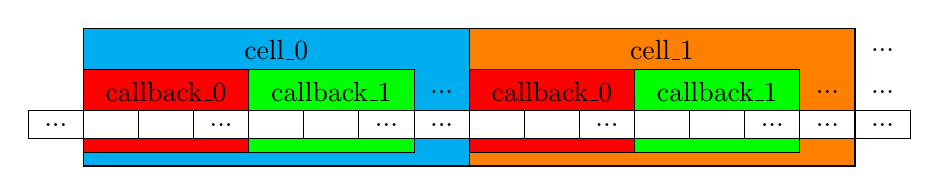
\begin{tikzpicture}[scale=0.7]
  % draw cells
  \draw[fill=cyan] (0,-0.5) rectangle ( 7,2);
  \draw[fill=orange]    (7,-0.5) rectangle (14,2);
  \node[align=center] at ( 3.5, 1.6) {cell\textunderscore{}0};
  \node[align=center] at (10.5, 1.6) {cell\textunderscore{}1};
  \node[align=center] at (14.5, 1.6) {...};
  
  % draw callbacks
  % cell_1
  \draw[fill=red]   (0,-0.25) rectangle (3,1.25);
  \draw[fill=green] (3,-0.25) rectangle (6,1.25);
  \node[align=center] at (1.5,0.85) {callback\textunderscore{}0};
  \node[align=center] at (4.5,0.85) {callback\textunderscore{}1};
  \node[align=center] at (6.5,0.85) {...};
  % cell_2
  \draw[fill=red]   ( 7,-0.25) rectangle (10,1.25);
  \draw[fill=green] (10,-0.25) rectangle (13,1.25);
  \node[align=center] at ( 8.5,0.85) {callback\textunderscore{}0};
  \node[align=center] at (11.5,0.85) {callback\textunderscore{}1};
  \node[align=center] at (13.5,0.85) {...};
  % beyond
  \node[align=center] at (14.5,0.85) {...};
  
  % draw contiguous memory
  \draw[fill=white] (-1,0) rectangle (15,0.5);
  \foreach \x in {0,...,14}
  \draw (\x,0) -- (\x,0.5);
  % cell_1
  \node[align=center] at ( 2.5,0.25) {...};
  \node[align=center] at ( 5.5,0.25) {...};
  \node[align=center] at ( 6.5,0.25) {...};
  % cell_2
  \node[align=center] at ( 9.5,0.25) {...};
  \node[align=center] at (12.5,0.25) {...};
  \node[align=center] at (13.5,0.25) {...};
  % beyond
  \node[align=center] at (-0.5,0.25) {...};
  \node[align=center] at (14.5,0.25) {...};
\end{tikzpicture}
\caption[Division of contiguous memory chunks for data transfer.]{Division of contiguous memory chunks for data transfer. Data is arranged according to the order of the cells. Registering \textit{pack} functions as callbacks allows to add multiple data chunks from different sources to each cell.}
\label{fig:memory}
\end{figure}

For the preparation of data buffers, all refinement indicators need to be terminally set. During both the packing and unpacking process, we determine whether cells will be or have been either refined, coarsened, or left untouched.

Simple data structures assigned on each cell can be easily packed and unpacked. On refined cells, we will distribute the same data from the parent on all children. However during coarsening, data needs to be merged from all children cells on the parent cell. Depending on the context, it is upon the user's decision to provide an appropriate strategy in this case, i.e.\@ the sum or average over all values, or to check whether data on all children is equal and choose these values.

However, the transfer of full finite element approximations is slightly more complicated. Here, we need to prepare data on each cell not only depending on the adaptation context, but also on the currently active finite element. In fact, we will already prepare data from the old mesh for the adapted grid in such a way that it just has to be unpacked on the new mesh. Regardless of whether \gls{cg} or \gls{dg} methods are employed, we will always store values of all \glspl{dof} on every cell to make sure that potential ghost cells will have access to all necessary data. \textcite{bangerth2012} developed an algorithm for transferring the solution across \h-adapted meshes in parallel, which we will expand to work with \hp-adaptation in the remaining part of this section.

Once all adaptation indicators have been set, we know how cells will change during the execution of refinement and coarsening, so a corresponding \textit{pack} callback will look as follows: On all active cells which will not be coarsened, we interpolate or project all \gls{dof} values of the currently active finite element to the future finite element. On nonactive cells which have active children that will be coarsened, we interpolate or project all \gls{dof} values from the currently active finite elements on children to the future finite element of the parent cell, which is determined as the encapsulating finite element space among all children (see Sec.~\ref{sec:adaptation}).

This way, all data has been prepared for the new mesh and has to be distributed on it with the following \textit{unpack} callbacks after \hp-adaptation happened and all \glspl{dof} have been enumerated on the updated mesh. On every active cell that has not been changed or that is the result of coarsening, we simply extract all \gls{dof} values. If an active cell is the result of refinement, we extract all \gls{dof} values from its parent cell and interpolate them on the refined cell. All extracted \gls{dof} values are left to be copied to the global data container corresponding to the finite element approximation.

In the following, we give a detailed description of the algorithm implemented in the \dealii{} library which is tied to the usage of \pforest{} \textcite{p4est22} as an oracle and relies on features provided by it. Here, the \dealii{} triangulation will be stored independently from the \pforest{} mesh.

In the application scope before adaptation is executed, users attach \textit{pack} callback functions to the triangulation and specify whether they qualify for fixed or variable size data transfer.

As soon as the user requests adaptation to be performed, all adaptation indicators will be carried over to the \pforest{} master mesh, which will be modified accordingly while maintaining the 2:1 mesh balance. The \dealii{} domain is left untouched.

We store a deep copy of the array of partition markers \parencite{burstedde2018} from the local \pforest{} object, which defines the global partition boundary allowing us to relate each cell to its corresponding subdomain. After repartitioning the \pforest{} master mesh, we know each cell's association to its subdomain on both the old and the adapted mesh with the corresponding partition markers, and thus source and destination processes for all \texttt{MPI} communication.

%And store its global first quadrant shared data structure from which we can determine the association of all processors to each cell, repartition the mesh among all processors, and store the same data structure again. This way we know each cell's association to a processor on both meshes. \parencite{burstedde2018}

%With the new global first quadrant data, we know for each cell which processes owned it on the old and the new mesh. We can thus perform the actual transfer as follows.

Comparing the meshes of the updated \pforest{} object with the \dealii{} triangulation lets us identify how cells have changed.
%This way, we can compare both and determine how cells have changed in the adaptation process.
With this information, we are able to prepare data from the old mesh for the new one. We create the contiguous memory buffers for fixed size and variable size data transfer, respectively, by triggering all callback functions that return buffers for the particular data on each cell. In addition, we will store how cells have changed with a corresponding flag and write it to the fixed size buffer.

We determine the sizes of every cell's data pack in each buffer. For fixed size data, we verify the equality of their size on all cells. We store a list with the data size of every cell from the variable size buffer. After that, the fixed size data buffer and the list of sizes from the variable size buffer will be communicated via the optimized fixed size transfer function provided by \pforest{} \parencite{burstedde2018}. Last, the variable size data buffer will be transferred using the analogously optimized function after the list of sizes is available on all processes.

%We will communicate the fixed size data buffer and a list of all sizes from the variable size data buffer via the optimized fixed size transfer function provided by \pforest{} \parencite{burstedde2018}. In a next step, variable size data will be transferred after the individual sizes are available.

%We could also send the variable data sizes with the fixed size data transfer. However for convenience, we keep it like this.

After adaptation has been performed and all data has been communicated, the user is left to reinitialize all data structures according to the updated mesh and \textit{unpack} the transferred data into them.

%We came up with the following code in application scope to perform data transfer across meshes: We will first register data to be transferred. Storing function pointers that deal with packing required data. We distinguish between fixed and variable size data.
%
%\begin{enumerate}
%\item Register.
%\item Prepare contiguous memory blocks.
%\item Perform fixed size data transfer.
%\item Perform fixed size data transfer for variable sizes.
%\item Perform variable size data transfer.
%\item Unpack data.
%\end{enumerate}

%We build continguous memory buffers for both fixed and variable size transfer, and store each size of the latter. Then, we transfer both the fixed size buffer and all sizes via fixed sized transfer. After that, we transfer the variable size transfer useing all sizes.

%When mesh is about to be

With this feature, we are able to send all sorts of cell related data across adapted meshes, i.e.\@ particle data, quadrature point data, and finite element approximations. Further, we use the above algorithm to transfer active finite element indices internally. To be more precise, future finite element indices will be sent and unpacked as active finite element indices on the adapted mesh.

These contiguous memory chunks can also be used for the purpose of serialization. In case the program shall be interrupted and resumed at a later stage, data will be dumped on the file system. We will create two separate files, each containing either fixed size or variable size data.

We need to determine the offset at which each process is supposed to write its local memory buffer into a global contiguous file. Thus, each process needs to know how much memory all preceding processes occupy. For fixed size data, this offset simply translates to the global index of the first cell on this process times the data size per cell. The global index can be determined from the array of partition markers of the \pforest{} object \parencite{burstedde2018}. However, in case of variable size data, we need to determine the offset with a prefix sum over the local buffer sizes of all preceding processes using \texttt{MPI\_Exscan}.

To resume the program successfully, we also need to store information about the data size of every cell, which we will prepend to the actual data in each file. In case of fixed size data, an integer corresponding to the data size per cell will be stored. For variable size data, we will collectively write the data size of every local cell in the global file, where each process's offset is determined by the global index of the first cell times the size of an integer.

Finally with these information, we can write all data collectively to the file system using \texttt{MPI\_File\_write\_at} \textcite{mpi31}, which can later be read via \texttt{MPI\_File\_read\_at} \textcite{mpi31}. For the serialization of the global mesh structure, we use the provided save and load functions of \pforest{}.

%With array of partition markers of the \pforest{} object \parencite{burstedde2018} combined with information about each cell's data size, we are able to determine the offset from the starting address that each processor needs to dump his data by a prefix sum over the cumulated data sizes.

%stores all cells in a consecutive order and partitions them, thus a sequence of all local cells across all processors

%to determine

%We need to find starting proc. Since we know the starting at the position of the global index of the first cell of the processor until the cumulated sum of the sizes on all locally owned cells.

Since all memory is written contiguously and the order of cells is independent of the partitioning, we can resume the program with a different number of processes as used during serialization.

%The preparation of data to be transferred and unpacking of transferred data has been realized in the \texttt{parallel::distributed::SolutionTransfer} \todo{cite} and \texttt{parallel::distributed::CellDataTransfer} classes within the \dealii{} library. The \texttt{parallel::distributed::Triangulation} \todo{cite} has been expanded by the preparation of the contiguous memory buffers and the execution of the transfer via \pforest{}.